
\chapter{Differentially Private Traffic Shaping}
\label{ch:dp-shaping}
% Chapter Introduction
Traffic shaping can be implemented at different layers within the network stack of an application.
At the transport layer, shaping involves dynamically adjusting the data transmission rate, specifically the size of data transmitted within a given time window, to ensure that the size and timing of data transmission do not disclose sensitive information of the applications.
At the network layer, traffic shaping is about transmitting packets in a manner that does not reveal users' private information through the timing and sizing of the packets. 
The selection of either approach has profound implications for both the design of shaping algorithm and the traffic shaping system itself.
Designing traffic shaping mechanism at network layer requires determining the size and transmission of every individual packets. 
Networking hardware capabilities, such as popular NICs, and network protocol specifications significantly constrain the design space in this context~\cite{mehta2022pacer}.  
On the other hand, to design a traffic shaping mechanism that operates on the top of transport layer, it is crucial to assume that \textit{after traffic shaping, the shaped traffic remains unaffected by the content or pattern of the unshaped traffic, during all subsequent processes such as encryption, packetization, and packet transmission scheduling}.
This assumption guarantees that the shaping mechanism maintains its integrity and effectively separates the sensitive information from the traffic pattern regardless the way network stack transmits the shaped traffic.
{\sys} performs differentially private traffic shaping on the top of transport layer, and in section {\addref} we elaborate on how our system satisfies this assumption.
 
The objective of our DP traffic shaping is to dynamically adapt the data transmission rate based on the available data stream, while simultaneously ensuring that the DP guarantees remain intact for any information that an attacker can observe, as specified in our threat model {\addref}.
We further extend 
The design of our traffic shaping algorithm relies on three key steps.
%
First, we formalize the information available to an attacker observing an application stream, which is all information such as packet sizes or timing at the finest granularity of observation.
We propose to use a buffering queue to collapse all this information into a sufficient statistic to adapt {\sys}'s transmission rate: the size of data in the queue waiting to be transmitted through our shaping mechanism.
%
Second, we show how to perform {\em DP measurements} of our buffering queue, in order to adapt \sys's transmission rate with DP guarantees.
We show that during data transmission with {\sys} shaping mechanism, the change of queue size is bounded, allowing us to perform DP measurements.
%
Third, we describe our decision mechanism for sending data based on DP decisions, which completes our DP shaping mechanism.
Intuitively, we can use DP queue measurements and public information such as network conditions to decide the amount of data to transmit.
Transmissions contain applications' queued data when some is available, and dummy data otherwise.
The traffic pattern observed by the attacker is a post-processing of the DP queries issued on the queue (depends on the private data only through the DP measurements), and is differentially private.


\section{Definitions and Assumptions}
\label{sec:dp-shaping-definitions}
An application's stream can be represented as a sequence of packets:
\begin{equation}
    \istream = \{{P^S_1}, {P^S_2}, {P^S_3}, \dots \}
\end{equation}
where ${P_i}^S = (l^S_i, t^S_i)$ indicates that the $i$\textsuperscript{th} input packet in $S$ has length $l_i$ bytes and is transmitted at timestamp $t_i$.
Without shaping, an adversary can precisely observe $\istream$ and infer the content, which is correlated with the~stream~\cite{schuster2017beautyburst}.

Our DP shaping relies on two key ideas.
First,~it models the DP guarantees for the (potentially long) traffic streams in windows of fixed length $\winlen$, denoted by \mbox{($\varepsilon_{\winlen}, \delta_{\winlen}$)-DP}.
An input sequence over window $j$ is a finite~sub\-sequence $S_{j} \subset S$, such that $S_{j} = \{ P^S_i~|~P^S_i \in S~and~t_i \in j \}$.
{\sys}'s DP guarantees cover all (overlapping) windows up to size $\winlen$.
A key assumption for {\sys}'s DP guarantees to hold over $\winlen$-sized windows is that the tunnel can always transmit all incoming data from application streams within any $\winlen$-sized time window.
In other words, we assume:
\begin{assumption}\label{assumption:window}
  All bytes enqueued prior to or at time $t$ are transmitted by time
  $t+W$.
\end{assumption}
We explain how to realize this assumption in a tunnel design in {\addref}.
Under this assumption, the privacy loss of the complete traffic stream is simply a DP composition of the privacy losses over consecutive windows.
The window length $\winlen$ is a configuration parameter, which is set before the start of an application's transmission. In practice, $\winlen$ would be in the order of a few seconds.

Secondly, we use the primitive of a {\em buffering queue} to control the maximum information accessible by an adversary within each window.
We denote the number of bytes present in the queue (\ie length of the queue) by $\qlen$.
Conceptually, {\sys} extracts bytes from the input stream, $\istream$, and enqueues them.
Furthermore, we discretize time into $\winlen$-sized windows and, at the beginning of each time window, {\sys} adds a DP noise to the queue length to determine the amount of data from the queue that should be transmitted as shaped traffic.
The shaped traffic is then transmitted as a packet sequence denoted by $\ostream$, which is observable by an adversary.
\begin{equation}
    \ostream = \{{P^O_1}, {P^O_2}, {P^O_3} \dots \}
\end{equation}
While shaping requires discretizing transmit windows, the DP guarantees apply over arbitrary windows.

In the rest of this section, we focus on {\sys}'s DP guarantees over a single window.
We first formally define a notion of ($\varepsilon_\winlen$,$\delta_\winlen$)-DP privacy, which guarantees DP over transmission windows of length $\winlen$.
The guarantee applies over all $\winlen$ windows, and applying DP composition yields guarantees over multiple windows.
Then, we provide an overview of the DP shaping mechanism, which further samples noise in multiple shorter uniform intervals within each window.
Finally, we prove how the shaping mechanism provides ($\varepsilon_\winlen$,$\delta_\winlen$)-DP.
To formalize {\sys}'s DP guarantees, we first define a meaningful distance between any pair of streams in windows of length $\winlen$ and the associated neighboring definition:

\begin{definition}
Two streams $S_{j}$ and $S_{j}'$ transmitted in a window $j$
are neighbors
%    if, within each time window $\window$,
if their L1-norm distance is at most~$\ssens$ bytes in a window of upto length $\winlen$, \ie ${\norm{~S_{j} - S_{j}'~}}_1 \leq \ssens$.
\label{def:neighboring-streams}
\end{definition}

$\ssens$ is the max L1-norm distance between each pair of application streams transmitted in any window $j$.
We utilize the L1-norm (the sum of absolute values) as our distance metric to quantify the dissimilarity between two traffic streams, as it captures differences in both packet sizes and temporal pattern.


\section{The Shaping Mechanism}
\label{subsec:dp-shaping-mechanism}
\paragraph{From windows to intervals.}
Based on \Cref{assumption:window} and \Cref{def:neighboring-streams}, the window length $\winlen$ affects the maximum number of bytes that can be accumulated in the buffering queue (thus, the maximum distance between stream pairs), as well as the transmission delay for the payload bytes enqueued.
Specifically, large windows lead to high-latency bursty traffic.
To reduce latency and burstiness, {\sys} further splits windows into smaller intervals of length $\dpintvl$ and samples noise at the beginning of each interval.
In absence of shaping, the queue length corresponds to the amount of unshaped traffic transmitted in an interval of $\dpintvl$.
The privacy loss over a window is now defined by applying DP composition on the privacy loss of individual intervals.

To apply noise in each interval, we now define the sensitivity of the queue  length over intervals of length $\dpintvl$.
Sensitivity, denoted $\qsens$, is the maximum difference in the queue length over any interval $\dpintvl$ that can be caused by changing one application stream to another.
Formally, consider two alternative streams $\streamw{j}$ and $\streamw{j}'$ passing through the queue.
Suppose that when transmitting $\streamw{j}$ (similarly $\streamw{j}'$), the queue length at the beginning of its $k$\textsuperscript{th} interval is denoted by $\qlent{k}$ (respectively $\qlent{k}'$). Then:
\begin{equation}
    \qsens = \max_{k = 0}^{\numupdates}~\max_{\streamw{j},
        \streamw{j}'} | \qlent{k} - \qlent{k}' |
    \label{eqn:ssens}
\end{equation}


\begin{figure}[t]
    \centering
    %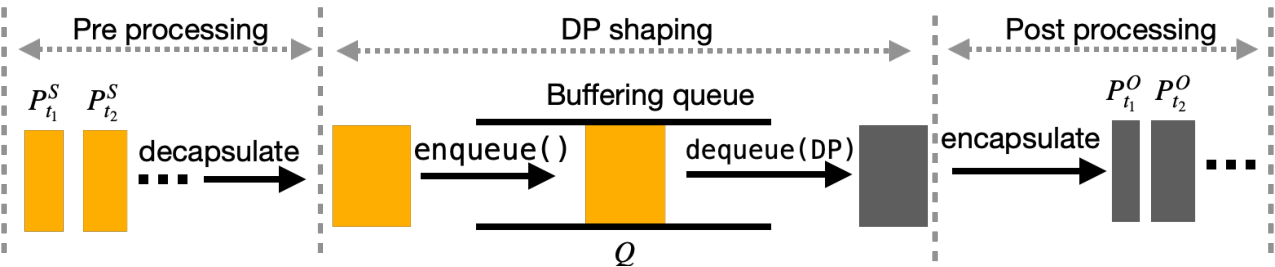
\includegraphics[width=\columnwidth]{figures/DPshaping_concept_vertical.pdf}
    %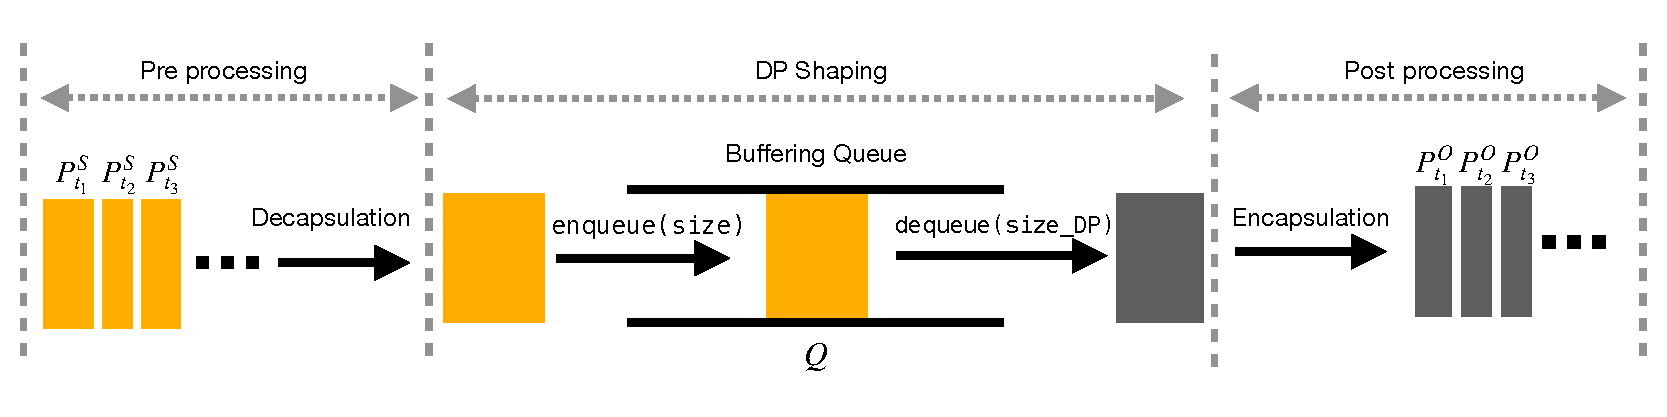
\includegraphics[width=\columnwidth]{figures/DPshaping_concept_horizontal.pdf}
    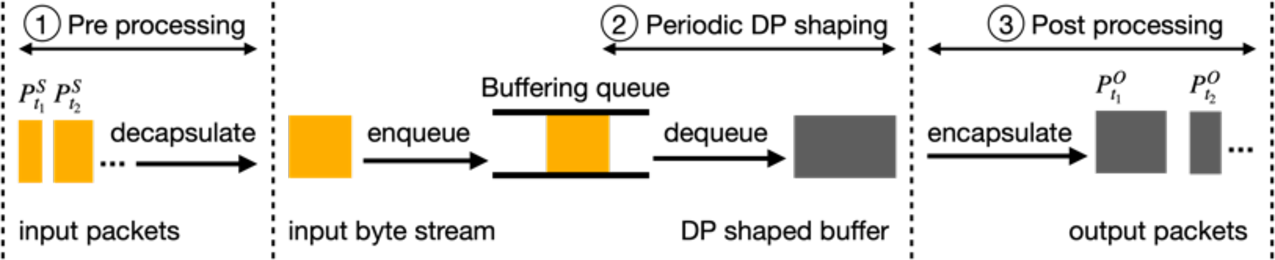
\includegraphics[width=\columnwidth]{figures/dp-overview.pdf}
    \caption{Overview of DP shaping}
    \label{fig:dp-overview}
\end{figure}

\paragraph{Shaping overview.}
\sys's DP shaping involves three steps as shown in \Cref{fig:dp-overview}.
\begin{enumerate}
    \item As application packets arrive in a window $\window$, the preprocessing step extracts the payload bytes and enqueues them into the buffering queue.
    \item In a periodic interval $k$, the core DP shaping algorithm performs a DP measurement, which entails sampling noise $z$ from a DP distribution and computing a DP burst size $\qlendpt{k} \triangleq \qlent{k} + z$.
    The shaping logic then prepares a {\em shaped buffer} of length $\qlendpt{k}$ with the application bytes available in the queue and dummy bytes if required.
    The DP shaping logic uses an additive Gaussian noise mechanism.
    The noise $z$ is sampled from a normal distribution $\mathcal{N}\big(\mu,~\sigma^2\big)$ parameterized by $\epsilon_\dpintvl$, $\delta_\dpintvl$, and~$\qsens$:
    The mean $\mu$ is 0 and the variance $\sigma^2$ is given by $\frac{2\qsens^2}{\varepsilon_\dpintvl^2}\ln(\frac{1.25}{\delta_\dpintvl})$.
    If the sampled noise is negative, we retain some of the data in the queue until the next DP measurement interval.
    Given this noise distribution, one measurement is \mbox{$(\epsilon_\dpintvl, \delta_\dpintvl)$-DP}.
    \item Data in the shaped buffer is then split into one or more packets and transmitted to the network. Since these packets are a post-processing of the DP-shaped buffer, they preserve DP as long as no new dependency on private data is introduced. 
    This last constraint requires the packets' size and transmit time to be selected independently of the data.
    We describe how {\sys} enforces this constraint in {\addref}.
\end{enumerate}
The privacy loss ($\varepsilon_{\winlen}$) and bandwidth overheads of the DP shaping (represented by $\sigma_\dpintvl$, \ie the standard deviation of the noise distribution function) depend on $\winlen$, $\ssens$, and the number of intervals $\varnumupdates = \numupdates$ in $\winlen$.
Additionally, the latency overheads depend on $\dpintvl$.
Note that for a specific value of $\ssens$ and $\varnumupdates$, the DP guarantee $\varepsilon_{\winlen}$ is fully specified by $\sigma_\dpintvl$, and remains the same even at different time scales.
That is, scaling $\winlen$ and $\dpintvl$ proportionally does not change the privacy and overhead costs.
We analyze the impact of different choices for these parameters on the privacy guarantees and overheads in \addref.
Here, we focus on a formal model of the DP guarantees.

\section{Privacy Guarantees}
\label{subsec:dp-shaping-guarantees}
At a high level, analyzing the  ($\varepsilon_{\winlen}, \delta_{\winlen}$)-DP guarantee of the overall shaping mechanism requires two steps:
\begin{enumerate}
    \item Showing that the difference in the buffering queue length is bounded for neighboring streams for all transmissions of the streams (\Cref{prop:sensitivity}).
    \item Composing the DP cost of each measurement over the intervals defining a window of length $\winlen$ (\Cref{prop:dp}).
\end{enumerate} 
We first show that the sensitivity of each measurement $\qsens$ is at most the window sensitivity $\ssens$:
\begin{proposition}\label{prop:sensitivity}
    {$\sys$} enforces $\qsens \leq \ssens$.
\end{proposition}
\noindent To prove the proposition stated above, we will first establish the following lemma.
\begin{lemma}
    Assume two neighboring traffic streams, $\streamw{j}$ and $\streamw{j}'$
    ($\|\streamw{j}-\streamw{j}'\|_1 \leq \ssens$), transmitted through {\sys}.
    If both streams are reshaped to the same output stream, $\ostream$, then by
    the end of any interval of shaping execution, the length of the buffering queue
    for the first and second streams are $\ssens$-close.
    In other words we have:
    
    \begin{equation}\label{equ:composition}
            \forall k \geq 0 : |\qlent{k} - \qlent{k}'| \leq \ssens
    \end{equation}
\end{lemma}

\begin{proof}
    {\sys} dequeues data from the buffering queue periodically at intervals of $T$
    seconds.
    Thus, while transmitting a stream $\istream$, the length of the buffering queue
    at the end of $k$\textsuperscript{th} interval, $\dpintvl_{k}$ is a function of
    three variables:
    \begin{enumerate}
            \item The length of the buffering queue at the end of
            $(k-1)$\textsuperscript{th} interval, $\qlent{k-1}$.
            \item The total number of payload bytes that have been dequeued from the
            buffering queue in the $k$\textsuperscript{th} interval,
            ${\payload}_{k}$.
            \item The number of new payload bytes from the application stream added
            to the buffering queue since the previous interval, which is the sum of
            sizes of all packets arriving between $(k-1)$\textsuperscript{th} and
            $k$\textsuperscript{th} interval, \ie
    %        $\sum_{T_{k-1} \leq t < T_k} P^S_t$
            $\sum_{\dpintvl_{k-1} \leq t < \dpintvl_{k}} P^S_t$.
    \end{enumerate}
    As two streams are reshaped to the output stream, $\ostream$, the DP burst size for two streams is the same in all intervals (i.e. $\forall k \geq 0 : \qlendpt{k} = \qlendpt{k}'$).
    
    Therefore, the length of the buffering queue after dequeue in the
    $k$\textsuperscript{th} interval is given by:
    \begin{equation}
    \qlent{k} =
    {\qlent{k-1}}
    +
    {\sum_{\dpintvl_{k-1} \leq t < \dpintvl_{k}} P^S_t}
    %{\sum_{T_{k-1} \leq t < T_k} P^S_t}
    -
    {{\payload}_{k}}
    \label{equ:queue-state}
    \end{equation}
    %\\
    Based on \Cref{equ:queue-state}, the difference between queue lengths of two
    neighboring streams, $\streamw{j}, \streamw{j}'$ at $k^{th}$ interval is:
    \begin{align}\label{equ:queue_state_expansion}
    & \qlent{k} - \qlent{k}'~=~(\qlent{k-1} - \qlent{k-1}')~+\\
    \nonumber
    & (\sum_{\dpintvl_{k-1} \leq t < \dpintvl_{k}}P^S_t - \sum_{\dpintvl{k-1} \leq t < \dpintvl_{k}}P^{S'}_t)
    -
    ({\payload}_{k} - {\payload}_{k}')
    \end{align}
    We divide the proof into two different steps.
    First, we show that the dequeue stage of the shaping mechanism does not increase the difference in queue lengths.
    Secondly, we show that under \Cref{assumption:window}, the enqueue stage of incoming streams does not increase the difference in queue lengths beyond $\ssens$.
    
    Suppose $\streamw{j}$ and $\streamw{j}'$ are reshaped to the same output stream,
    $\ostream$. Thus, the sizes of output packets generated in each decision
    interval $\dpintvl$ when transmitting either streams is the same. However, the
    content of the output packets in each stream may differ based on the sizes and
    timing of the packets in each input stream.
    For the shaping mechanism, this implies that the number of payload bytes
    dequeued from the buffering queue for when transmitting each stream may not
    necessarily match.
    %This is because one queue might not have a sufficient amount of traffic to meet
    %the requirements of the DP decision, resulting in the need to add dummy traffic.
    Nevertheless, the shaping mechanism always satisfies the following inequality:
    
    \begin{equation}\label{equ:queue-dequeue}
            (\qlent{k} - \qlent{k}').({\payload}_{k} - {\payload}_{k}') \geq 0
    \end{equation}
    %As we mentioned before, the $\qlent{k}$ determines the size of the queue after
    %$\payload_k$ bytes of data are dequeued from the queue.
    
    To show why \Cref{equ:queue-dequeue} always holds, we consider all
    the possible scenarios for two queue lengths after $k$\textsuperscript{th}
    interval:
    \begin{enumerate}
        \item $\qlent{k}$, $\qlent{k}' > 0$: 
        This indicates that there are still some untransmitted payload bytes remaining in the buffering queue for both streams. 
        Consequently, it implies that the shaping mechanism does not add any dummy bytes to compensate for the difference between the DP burst size and the amount of data in the queues.
        We also know that the DP burst size for two streams are the same ($\qlendpt{k} = \qlendpt{k}'$)
        Therefore: ${\payload}_{k} = {\payload}_{k}' \rightarrow {\payload}_{k} -
        {\payload}_{k}' = 0$.
        \item $\qlent{k},~\qlent{k}' = 0$: This simply implies $\qlent{k} -
        \qlent{k}'=0$
        \item $\qlent{k} = 0,~\qlent{k}'>0$: The DP burst size is the
        same for both
        queues. Thus, the first queue provided less payload data since it has emptied
        out. This means: ${\payload}_{k} \leq {\payload}_{k}'$.
        \item $\qlent{k}' = 0,~\qlent{k}>0$: This is symmetric to the previous case.
    %    With the same of justification of previous case we have:
    %    ${\payload}_{k} \geq {\payload}_{k}'$
    \end{enumerate}
    Now, using \Cref{equ:queue-dequeue}, we prove the following:
    \begin{align}
            |\qlent{k} - \qlent{k}'|
            \leq
            |\qlent{k-1} - \qlent{k-1}'|
            +
            \sum_{\dpintvl_{k-1} \leq t < \dpintvl_{k}}|P^S_t - P^{S'}_t|
    \end{align}
    Let's consider $(\qlent{k}-\qlent{k}') \geq 0$. (The case of
    $(\qlent{k}'-\qlent{k}) \geq 0$ is symmetric.)
    % \footnote{The proof is similar for the case of $(Q_{i}-Q_{i}') \leq 0$.}
    %We can rewrite Equation (\ref{equ:queue_state_expansion}) as follows:
    %\am{How do we add the absolute to equation 5?}
    Using Equation (\ref{equ:queue_state_expansion}), we get:
    \begin{align*}
    \nonumber
    & |\qlent{k} - \qlent{k}'| = \qlent{k} - \qlent{k}'\\
    & = (\qlent{k-1} - \qlent{k-1}')
    +
    (\sum_{\dpintvl_{k-1} \leq t < \dpintvl_{k}}P^S_t - P^{S'}_t) - ({\payload}_{k} -
    {\payload}_{k}')
    \\
    & \leq
    (\qlent{k-1} - \qlent{k-1}')
    +
    (\sum_{\dpintvl_{k-1} \leq t < \dpintvl_{k}}P^S_t - P^{S'}_t)
    \\
    & \leq
    |
    (\qlent{k-1} - \qlent{k-1}')
    +
    (\sum_{\dpintvl_{k-1} \leq t < \dpintvl_{k}}P^S_t - P^{S'}_t)
    |
    \\
    & \leq
    |\qlent{k-1} - \qlent{k-1}'|
    +
    \sum_{\dpintvl_{k-1} \leq t < \dpintvl_{k}}|P^S_t - P^{S'}_t|
    \end{align*}
    Intuitively, this means the dequeue stage, never increases the difference
    between two queues lengths.
    Now, we show that under \Cref{assumption:window}, the difference in queue lengths is bounded.
    \\
    With $d_k = |\qlent{k}-\qlent{k}'|$ and $d_0 = 0$, we have:
    \begin{align}
    \nonumber
    & d_k \leq d_{k-1} + \sum_{\dpintvl_{k-1} \leq t < \dpintvl_{k}}|P^S_t - P^{S'}_t|\\
    &~~~=
    \nonumber
    0 + \sum_{i=0}^{k}\big({\sum_{\dpintvl_{i-1} \leq t < \dpintvl_{i}}|P^S_t - P^{S'}_t|}\big)\\
    &~~~=
    \nonumber
    \sum_{0 \leq t < \dpintvl_{k}} |P^S_t - P^{S'}_t|\\
    \nonumber
    &~~~= \sum_{0 \leq t < \dpintvl_k - W} |P^S_t - P^{S'}_t| +
    \sum_{\dpintvl_{k} - W \leq t < \dpintvl_{k}} |P^S_t - P^{S'}_t|\\
    \nonumber
    &~~~=
    0 + \|\streamw{j} - \streamw{j}'\|_1
    \leq
    \ssens
    \end{align}
\end{proof}
\noindent To conclude, the maximum difference between queue lengths (\ie the sensitivity,
$\qsens$) is always bounded by $\ssens$.
\begin{align}
        \qsens = \max_{k = 0}^{\numupdates}~\max_{\streamw{j},
        \streamw{j}'} | \qlent{k} - \qlent{k}' | \leq \ssens
\end{align}
We can then reason about DP guarantees over intervals of length $\dpintvl$ in
order to achieve the privacy loss for the entire window of length $\winlen$.
%
Formally, we have:
\begin{proposition}\label{prop:dp}
    {$\sys$} enforces $(\varepsilon_{\winlen}, \delta_{\winlen})$-DP, 
    \\ 
    with $\varepsilon_{\winlen}, \delta_{\winlen} \triangleq
    \textrm{DP\_compose}(\varepsilon_T, \delta_T, \numupdates)$.
\end{proposition}
\begin{proof}
    By Prop. \ref{prop:sensitivity}, the sensitivity of each measurement is at most $\ssens$.
    By the Gaussian DP mechanism, the measured queue size $\qlendpt{k}$ in each interval $k$ of length $\dpintvl$ is $(\varepsilon_{T}, \delta_{T})$-DP.
    Using DP composition over $\numupdates$ $(\varepsilon_{T}, \delta_{T})$-DP measurements, and the fact that $\ostream$ is a post-processing of DP measurements, yields the ($\varepsilon_{\winlen}, \delta_{\winlen}$)-DP over any $\winlen$ length window.
\end{proof}
We use R\'enyi-DP composition on the Gaussian mechanism for $\textrm{DP\_compose()}$.
Note that the overhead (\ie noise added) due to DP does not depend on the number of streams: the overhead is the same regardless of the number of streams transmitted through the buffering queue simultaneously.


